\documentclass[aps,rmp,reprint,amsmath,amssymb,graphicx,longbibliography]{revtex4-1}

\usepackage{bm}
\usepackage{graphicx}% Include figure files

\newcommand{\vq}{{\vec q}}
\newcommand{\vf}{v_{\rm F}}
\newcommand{\kf}{k_{\rm F}}
\newcommand{\Phio}{\Phi_0}
\newcommand{\tp}{t_\perp}
\newcommand{\Hca}{\mathcal{H}}
\newcommand{\vk}{{\bf k}}

\begin{document}

\title{The Quantum Internet --- Towards the Singularity}

\maketitle






\subsection{Applications of a space-based quantum network}

\subsubsection{Quantum key distribution}

As we have discussed in Sec. [TB:please fill this in], the demand for secure cryptography is now extremely important in the context of electronic commerce and general security of information transmission in the internet age. Electronic currencies such as Bitcoin depend on cryptographic protocols in order to secure the value of the assets, assign ownership, and secure the currency against fraud.  However such protocols are based upon computational complexity of certain mathematical problems, and are not fundamentally secure in the presence of limitless computational resources, or quantum computers.  Therefore, using quantum mechanical protocols which are based on physical principles rather than computational limitations, are favorable in the sense of future-proofing the security.  Quantum key distribution is a relatively mature technology with already several commercial systems being available.  The main drawback is thus the ability to perform long-distance transmission of photons.  For these reasons, current quantum key distribution networks have been limited relatively small area in the region of $ \sim $ 100 km, such as in Austria, Switzerland, Japan, USA, and China \cite{lo2014secure}.   The longest distance QKD network that is currently planned is the Beijing to Shanghai quantum key distribution link spanning a distance of 2000 km.  This involves 32 trusted nodes to break the total distance into shorter segments to convert the quantum information to classical information.  

Utilizing space communications for the purpose of quantum key distribution has been discussed in several works \cite{hughes2000quantum,rarity2002ground,pfennigbauer2003free,aspelmeyer2003long,armengol08}. As already demonstrated in the space entanglement  experiments \cite{yin2017satellite,ren2017ground,liao2017satellite} far lower attenuation rates are possible using the technique that in either free space or optical fiber methods.  Since cryptography schemes such as BB84 do not require entanglement, these would appear to be the first commercial widespread application of quantum technologies.  The high feasibility of space based quantum key distribution was already noted in a variety of configurations including ground-to-space and space-to-ground quantum communication \cite{rarity2002ground,aspelmeyer2003long}.  In the context of security, the first long-distance experiments that are likely to be performed employing trusted nodes.  For example, after performing quantum key distribution between satellite and a ground station, a satellite could store the key for some time until another quantum key distribution can be performed to another ground station using a one-time pad \cite{liao2017satellite}.  These types of experiments are planned eventually to perform intercontinental quantum key distribution between China and Austria.  









\subsubsection{Quantum clock synchronization}


Clock synchronization is a fundamental task that is has widespread applications, ranging from navigation, telecommunications, financial transactions, the internet, and many scientific applications. Of these, the Global Positioning System (GPS) has become a day-to-day necessity for a large fraction of the human population as it has been increasingly built into smartphones and other devices. The GPS system famously relies upon very precise clock synchronization to perform its task through a process of quadrangulation from several satellites. Due to the high speed of light, one requires in practice highly synchronized clocks which are accurate to a centralized time standard to the $\sim$ ns level. This allows positioning to be performed to the $\sim$ m level, which is acceptable for many applications. GPS satellites have atomic clocks that are stable to one part in $10^{13}$, so that active corrections can maintain the accurate to the $\sim$ ns level. The great success of the GPS system in turn has created a further demand for increasingly precise navigation. For example, autonomous vehicles would immediately benefit from a more precise navigation system. In principle, technology for more stable clocks is already present, with atomic clocks exceeding stabilities of those on satellites being routinely produced, and optical atomic clocks now reaching stabilities of one part in $10^{18}$  \cite{ludlow2015optical}. An outstanding question is then how to synchronize these clocks given their remarkable stabilities. 


\begin{figure}
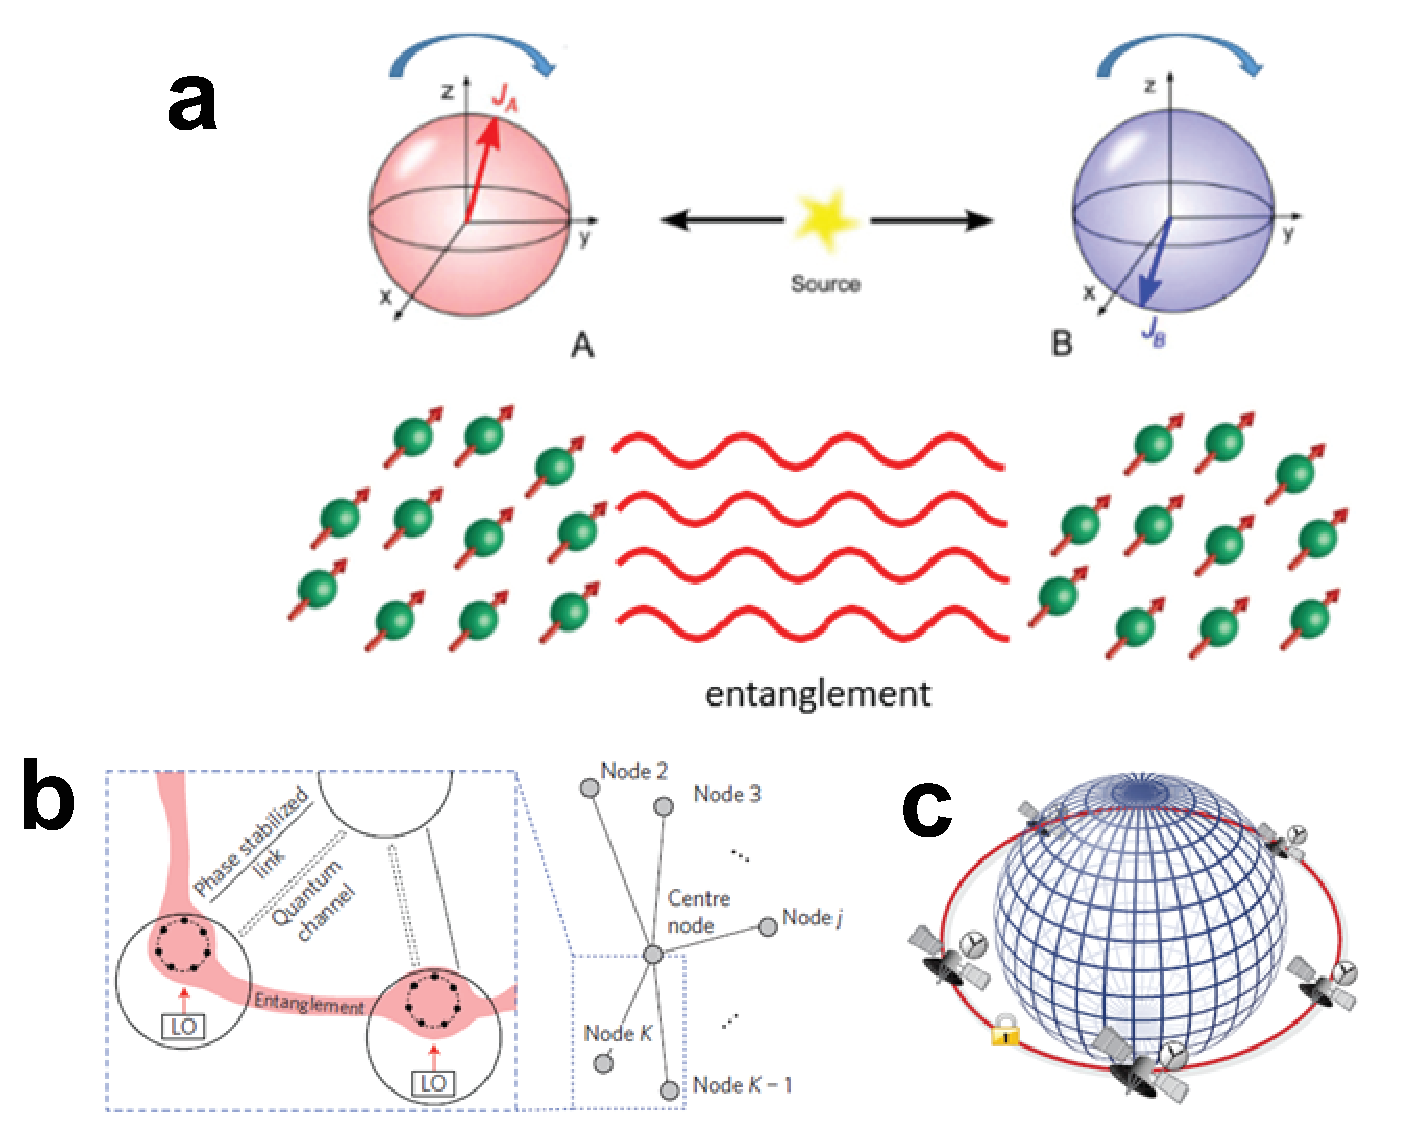
\includegraphics[width=\columnwidth]{figspace3}
\caption{Quantum clock synchronization schemes. (top) The proposal by Jozsa, Dowling, and co-workers where a singlet state is shared and measured in an ensemble of qubits \cite{jozsa00}. (bottom) The proposal by Lukin, Ye, and co-workers where a GHZ state is generated between satellites to obtain measure the frequency drift at the Heisenberg limit \cite{komar14}. }
\label{figspace3}
\end{figure}



Several past works have examined the problem of clock synchronization in space (see also Sec. [TB: refer to other section on clock sync]). In the proposal of Jozsa and co-workers, many copies of shared entanglement in a singlet state is first distributed and stored on the clock states of an atomic clock \cite{jozsa00}.  The measurement is then made by one of the parties, which collapses the states simultaneously at each party, and the time evolution of the states begins. Classical information is exchanged between them, which reveals the time elapsed since the measurement, which can be used to synchronize the clocks. While the original protocol only allowed allowed clock synchronization between two parties, similar ideas were used to extend it to a multiparty context \cite{krvco2002quantum,ben2011optimized,ren2012clock}.  In a more recent proposal, a shared GHZ state is prepared across all the nodes of the quantum network, which allows for a quantum metrologically enhanced detection of the clock signal drift at the Heisenberg limit \cite{komar14}. The use of shared resources acts to improve the overall precision, allowing for an optimal scheme for the qubit resources that are used. Several other proposals have also been made, which are quantum versions of Eddington's slow clock transport where the qubit keeps time of the transmission time \cite{chuang2000quantum,tavakoli2015quantum}. 

Experimentally, there have been several demonstrations of the protocol, albeit at relatively short distances.  Continuous time-bin entangled photons were used as the entanglement resource to obtain a time-correlation between a distance of 3 km \cite{valencia2004distant}, and another technique based on Hong-Ou-Mandel interferometry was performed with a 4 km fiber link \cite{quan2016demonstration}.  Several other demonstrations based on NMR \cite{zhang2004nuclear,kong2017implementation} have also been performed. 

There are however several outstanding problems with the quantum clock synchronization scheme as presented above. In the scheme of Jozsa and co-workers, if one starts in a perfect singlet state, the scheme works as intended, but if one instead starts in the state 
%
\begin{align}
\frac{1}{\sqrt{2}} \left( | 0 \rangle_A | 1 \rangle_B - e^{i \delta} | 1 \rangle_A | 0 \rangle_B \right)
\end{align}
%
then one obtains an offset to the synchronizations between the two parties. In practice, such a phase could arise from decoherence induced noise, or differences in the basis conventions that the two parties choose. Thus in practice entanglement purification would to be performed to produce a singlet state with $ \delta = 0 $ before the synchronization protocol is performed.  However, it was argued that to perform the entanglement purification quantum circuit correctly, the timing of the quantum gates would need to be controlled, which requires synchronized clocks \cite{preskill2000quantum} --  rendering the syncrhonization impossible. It was previously been shown that such a phase cannot be eliminated using asynchronous entanglement purification \cite{yurtsever02}, and hence the protocol remains incomplete in the general case where imperfect singlet pairs are shared. 








\subsubsection{Fundamental physics experiments}

The availability of a globe-spanning quantum network on satellites brings the opportunity for fundamental quantum mechanical experiments and unprecedented length scales and velocities in the future.  Satellite-to-satellite photon transfer can allow for ultra-long distance quantum communications that are not possible on Earth due to atomospheric loss.  Another unique aspect of space is that the satellites are moving at high velocity –- typically at $10^{-5} $ times the speed of light for low Earth orbit satellites.  The combination of both of these effects gives a unique opportunity for performing relativistic quantum information experiments to test fundamental physics. 

We anticipate that some of the first choices of experiments will be extensions of what are already performed on Earth.  For example, one can perform increasingly long space-based Bell violation tests at unprecedented distances \cite{yin2017satellite}.  Another possibility is to examine the speed of influence of entanglement, which bound the speed of entanglement \cite{yin2013lower}.  In space, such experiments could be extended much further, giving tighter bounds.  There are demanding technical hurdles that must be overcome to accomplish such experiments, such as the necessity of synchronized clocks. In addition to examining extensions of existing experiments, the high satellite velocities can be used to perform relativistic quantum information experiments, such as entanglement tests in the presence of special and general relativity, Wheeler's delayed choice experiment, and enhanced quantum metrology \cite{kaltenbaek2003proof,scheidl2013quantum,ahmadi2014relativistic}.  










\bibliography{references}

\end{document}
